% This is the aspauthor.tex LaTeX file
% Copyright 2010, Astronomical Society of the Pacific Conference Series

\documentclass[11pt,twoside]{article}
\usepackage{asp2010}

\resetcounters

%\bibliographystyle{asp2010}

\markboth{Jun-Hui Zhao}{Miriad for SMA Data Reduction}

\begin{document}

\title{Miriad for SMA Data Reduction}
\author{Jun-Hui Zhao
\affil{Harvard-Smithsonian CfA, MS 78, 60 Garden Street., Cambridge, MA02138 }}

\begin{abstract}
Multichannel image reconstruction, image analysis, and display ({\it Miriad}) 
is a command line based software package, originally developed to handle 
data from the BIMA millimeter array telescope. The software package has been 
adapted for the reading, calibration, and imaging of the Submillimeter Array
(SMA)  data. In this conference, we report and outline the data reduction
procedure that has been used for processing SMA data with the {\it Miriad} 
software. 	 
\end{abstract}

\section{The Submillimter Array}
The Submillimeter Array (SMA)\footnote{The Submillimeter Array is a joint 
project between the Smithsonian
Astrophysical Observatory and the Academia Sinica Institute of Astronomy
and Astrophysics and is funded by the Smithsonian Institution and the
Academia Sinica.} is an 8-element radio interferometer located atop Mauna Kea 
in Hawaii. Operating at frequencies from 180�GHz to 700�GHz, the 6m dishes 
may be arranged into configurations with baselines upto 509m, producing a 
synthesized beam of sub-arcsec. Each element can observe with two receivers 
simultaneously, with 2�GHz bandwidth each. The digital correlator backend 
allows flexible allocation of thousands of spectral channels to each receiver.

\section{Miriad for SMA Data Reduction}
{\it Miriad} is a radio interferometer data reduction package \citep{stw95} 
and has been adopted by the SMA for data reduction.\footnote{http://www.cfa.harvard.edu/sma/miriad/} {\it Miriad} can be configured 
for the specifications required by the SMA. Specific codes for handling 
the SMA data have been developed and are supported. {\it Miriad} now can be 
used for the reduction of continuum and spectral line observations from 
loading of the SMA archival data  through to the image analysis.�The SMA 
features have particular emphasis on aspects of interest to users of the 
SMA. We support the off-line software including software tools used for 
calibration and analysis of the SMA data observed at submillimeter 
wavelengths. The newly developed codes are (will be) placed under 
{\it Miriad} CVS system (./miriad$_{-}$cvs/src/prog/sma) 
which is managed by the CARMA group.�

\begin{figure}
\centering
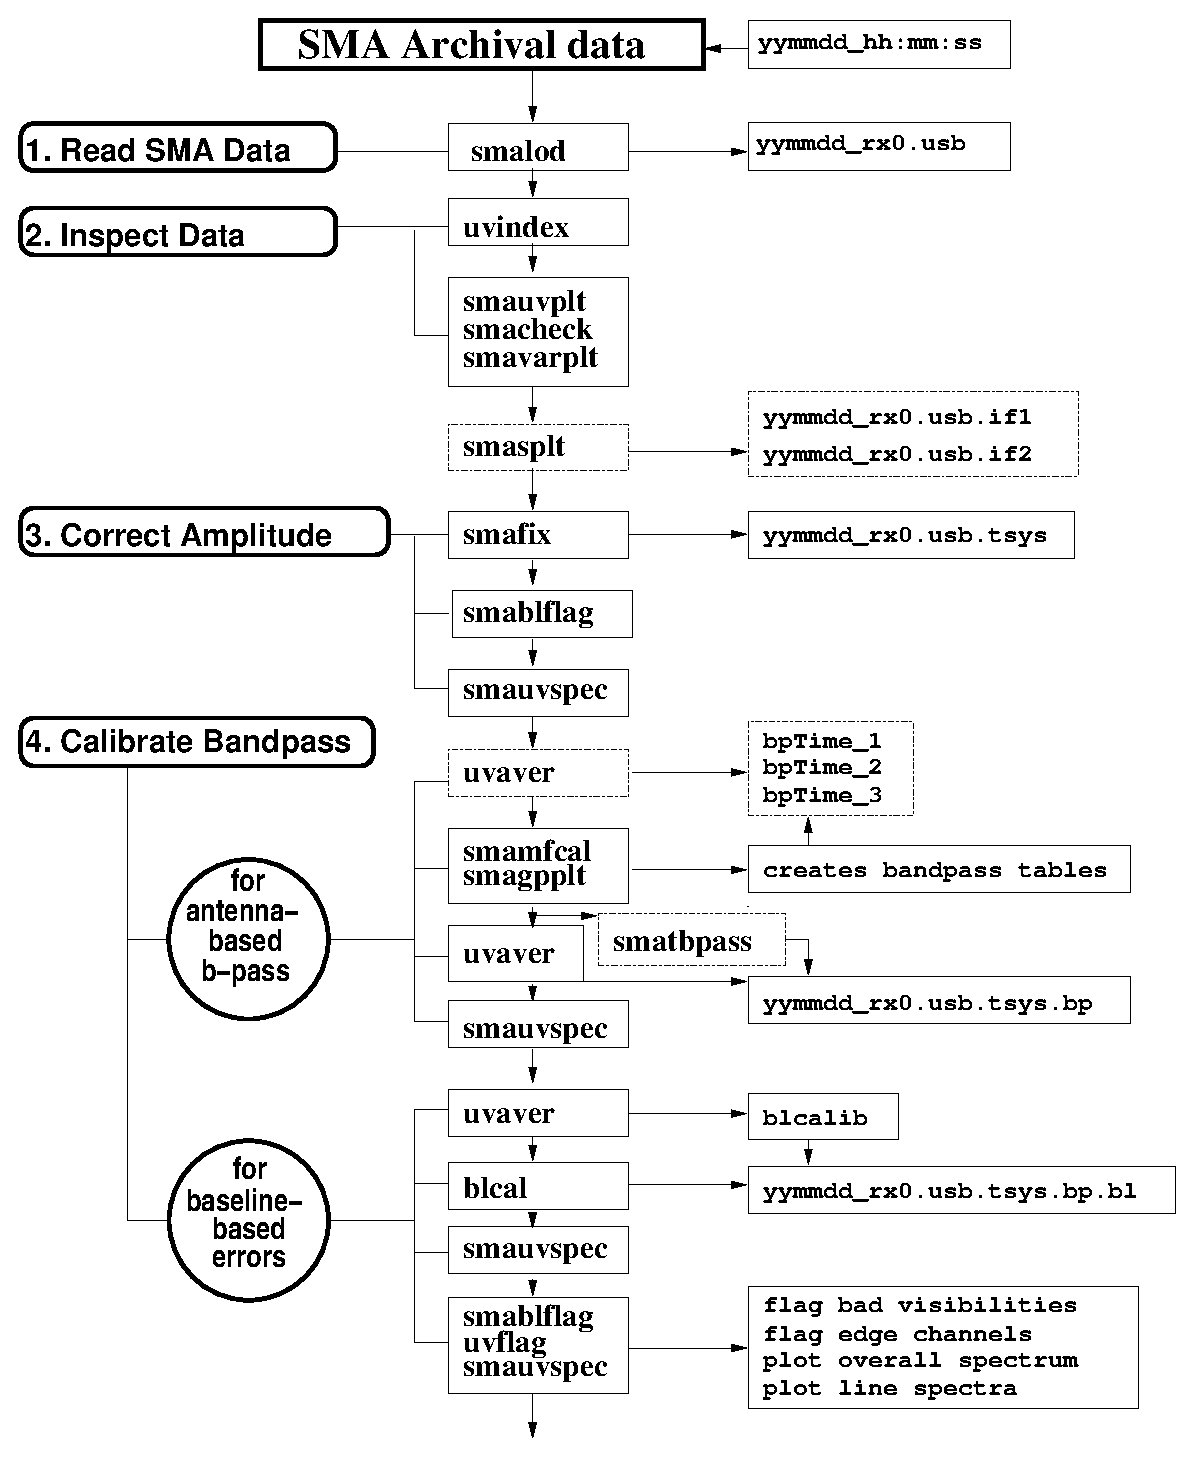
\includegraphics[scale=0.5, angle = 0]{f1a.eps}
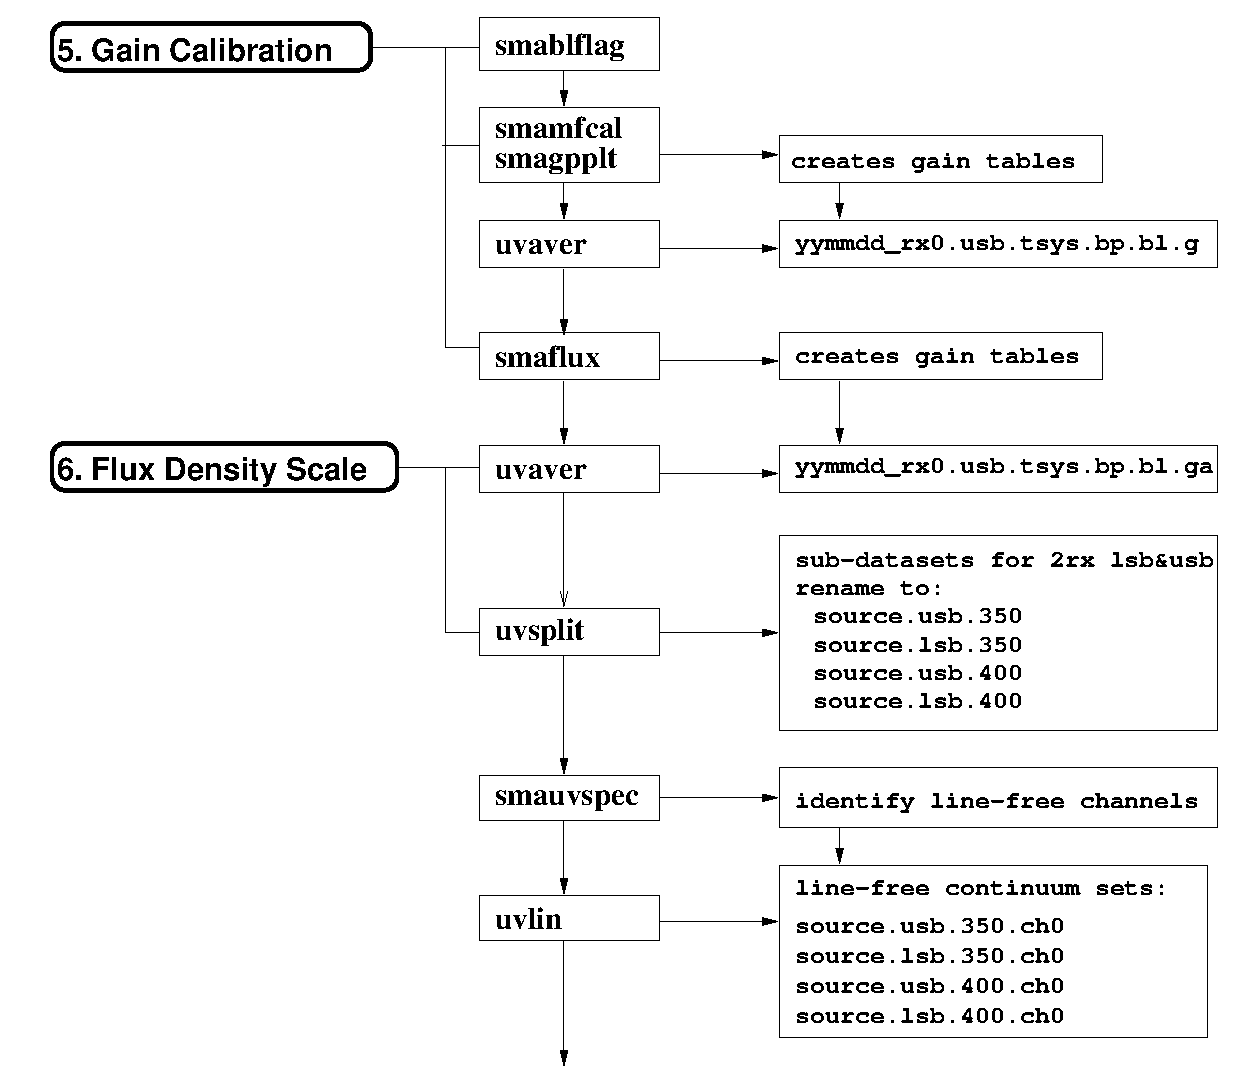
\includegraphics[scale=0.5, angle = 0]{f1b.eps}
\end{figure}
\begin{figure}
\centering
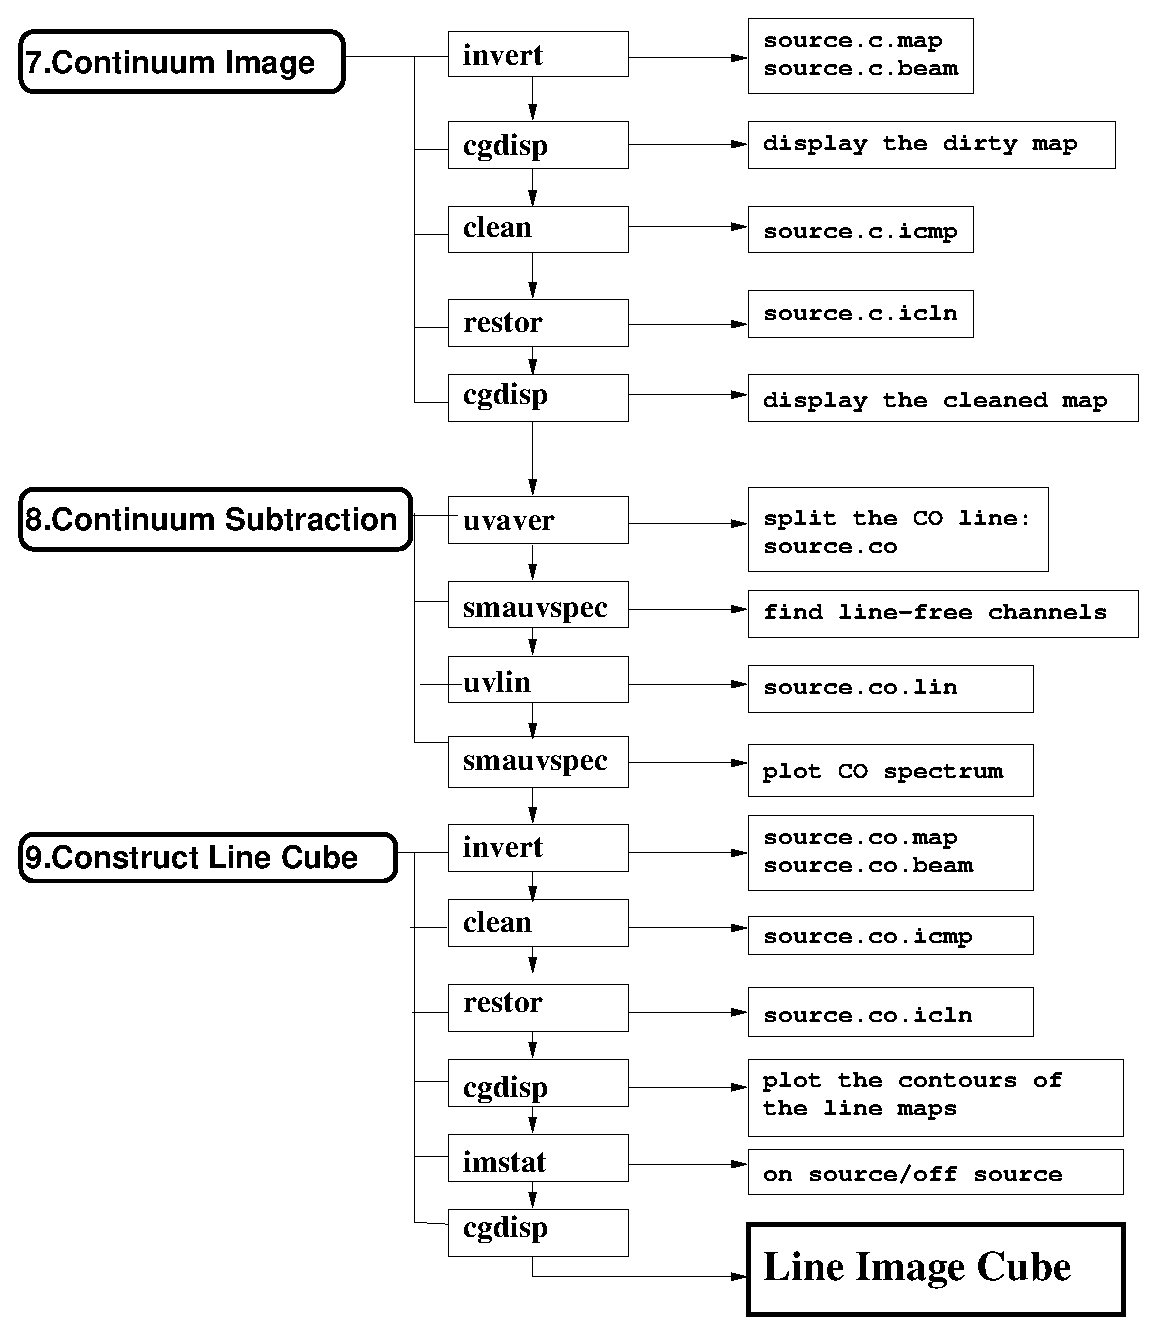
\includegraphics[scale=0.5, angle = 0]{f1c.eps}
\caption{A flow chart of handling SMA data in {\it Miriad}.
{\it Left column} shows the major steps of the data reduction
procedure. {\it Middle column} lists the {\it Miriad} tasks used in
the process. {\it Right column} shows the final calibrated uv
data and image files as well as the interim uvdata, gain
table and image files produced from the data reduction
process.}
\end{figure}

\begin{figure}
\centering
\begin{minipage}{20pc}
\centering
\includegraphics[height=0.137\textheight,angle=-90]{f2a.ps}
\includegraphics[height=0.155\textheight,angle=-90]{f2c.ps}
\end{minipage}
\vspace{0pc}
\begin{minipage}{20pc}
\centering
\includegraphics[height=0.155\textheight,angle=-90]{f2b.ps}
\includegraphics[height=0.137\textheight,angle=-90]{f2d.ps}
\end{minipage}
\caption{The result plots produced from one of the example scripts 
based on SMA observations of DM Tau.
{\it Top-left}: a continuum image of DM Tau made with the data from LSB 
and USB of both 350 and 400 receivers.
{\it Bottom-left}: a spectrum of USB from 350 GHz receiver.
{\it Top-right}: a CO(3-2) line profile.
{\it Bottom-right}: an image of integrated CO line emission from DM Tau. }
\end{figure}


\subsection{Powered for Submillimeter Data Reduction}

SMA planet models have been used for flux density scale calibration 
for the submillimeter observations in {\it Miriad}.\footnote{Mark Gurwell, 
http://sma1.sma.hawaii.edu/planetvis.html}
The SMA planet models have been coded in {\it smaflux}.
Also,  {\it smamfcal} is implemented with 
running-smooth and polynomial fitting algorithms 
to enhance the S/N for weak bandpass calibrators, 
and visibility-intensity weighting to weight down 
the lower S/N visibilities in the case of a resolved 
planet disk source to be used as bandpass calibrator.
Various plotting tasks are implemented with color 
indices for identifying sources, spectral windows, and 
polarization components.

\subsection{A Step-by-step for SMA Data Reduction}
A step-by-step procedure for the reduction of both SMA continuum 
and spectral line data can be summarized by nine major steps: 
1) read the archival data; 
2) inspect data; 
3) corrections for system temperature; 
4) bandpass corrections; 
5) complex gain calibration; 
6) flux-density scale calibration; 
7) imaging continuum emission; 
8) continuum subtraction; 
9) Construction of spectral line cube. Fig. 1 shows a flow chart
of processing SMA data in {\it Miriad} from reading data, calibrations
to final images.

\subsection{Tutorial Scripts }
One of the nice features in {\it Miriad} is that the detailed 
procedure of input setup and execution of data reduction tasks 
can be compiled in a shell script program. SMA staff have taken 
the advantage to provide users tutorial examples in C-shell 
scripts for reducing data acquired from the basic observing 
modes including hybrid-spectral resolution, dual receivers, 
polarization, mosaic with the standard SMA correlator configurations 
(2GHz bandwidth) or the double-band modes (4GHz bandwidth). 
The examples of the scripts have been posted on the SMA-Miriad 
webpage.\footnote{http://www.cfa.harvard.edu/sma/miriad/spec/SMAscripts/}
Fig. 2 shows the result plots from one of the example scripts 
(a non-polarization, 2 receiver mode) based on the test data 
from observations of DM Tau.

\section{Future Plan}
In the near future, the SMA backend will be implemented with a broad-band digital
correlator producing  tens of thousands of spectral  channels to each receiver.
A typical size of data produced from an observing track will exceed 50 Gbytes. 
{\it Miriad} can be adapted for the SMA upgrade.  

\acknowledgements The article was presented by JHZ on behalf of the SMA
team and {\it Miriad} developers. JHZ is grateful to Mel Wright, Peter
Teuben \& Bob Sault for their contributions in supporting SMA data reduction 
with {\it Miriad}. 

%\bibliography{aspauthor}
\begin{thebibliography}{}
\bibitem[Sault, Teuben \& Wright (1995)]{stw95}
Sault, R. J., Teuben, P. J. \&  Wright, M. C. H, 1995, in {\it Astronomical Data Analysis Software and Systems IV}, ed. by R.A. Shaw, H.E. Payne, 
\& J.J.E. Hayes, ASP Conference Series, Vol. 77, p433
\end{thebibliography}

\end{document}
